\chapter{Design}\label{ch:Design}

\section{Introduction}
\subsection{Problem Definition and outline}
In many types of datasets, a class imbalance is frequent as there are much fewer incidences of the target outcome label than of the "normal" ones . Class imbalance in data  can lead algorithms to misidentified instances, giving a "normal" label to a target instance, for example, because the data on which the algorithm was trained did not contain enough instances of the "target" label.  There are many real-life instances where the wrong classification of an instance could have devastating consequences and the aim of this project is to:
\begin{enumerate}
\item compare the performance of several different algorithms on imbalanced datasets
\item identify potential solutions that will allow the algorithms to "learn more efficiently" even when a class is underrepresented
\item test the different solutions and compare the performance of the algorithms on the same datasets once the solutions have been implemented
\end{enumerate}
\subsection{Class Imbalance in healthcare datasets}
Healthcare-related datasets are particularly sensitive to the class imbalance problem and this can be more or less severe depending on the condition that is being studied. Some diseases have a more frequent occurrence than others, for example certain types of cancer have a very low incidence, especially when looking at the general population, while others are much more common, though their incidence in the population at large will still create a class imbalance. There are however situations where the class imbalance is reversed and incidence of "sickness" tends to be higher than that of "health", and this has been reported in EHR data; since EHR data are formed from doctors' patient records, there tends to be an over-representation of unhealthy cases versus healthy ones in those dataset. In either case, the intrinsic bias of the data towards one of the classes will create issues when training an algorithms as there are insufficient cases of one class to learn from. This will likely result in the algorithm failing to identify properly cases of "sick" label for example and mislabelling them as "healthy". This problem could be further amplified if the class distribution in the data used for training is very different from the class distribution in the testing or live data, on which the algorithm will be used.
In cases of medical diagnostic this could have dramatic consequences as the wrong diagnosis could be issued to a patient. 

\subsection{Proposed solutions}

what are the known solutions to the problem
\subsection{Experimental design outline}


\begin{figure}[H]
    \centering
    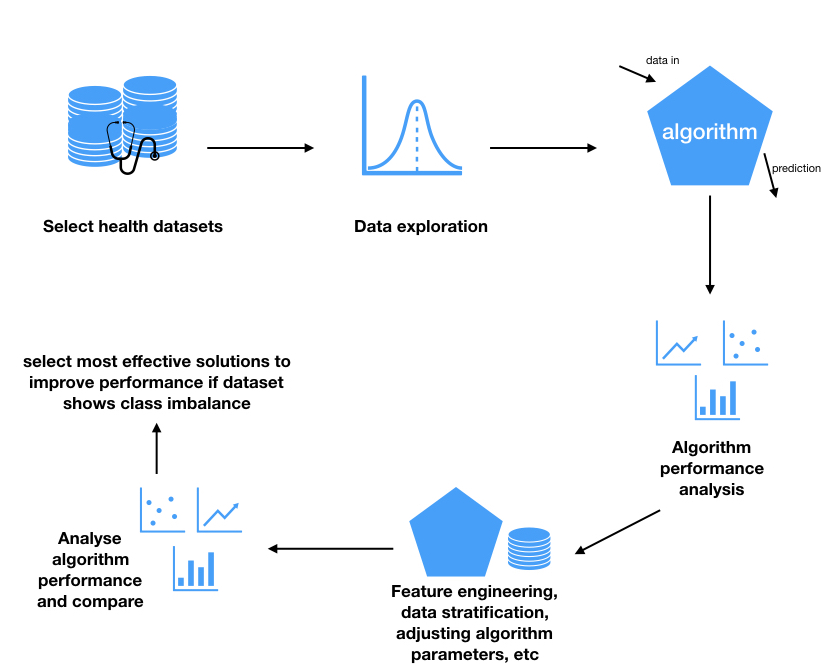
\includegraphics[width=0.8\textwidth]{ThesisTemplate/usingLatex/images/Chapter3Figures001.jpeg}
    \caption{Schematic of the experimental design of the study.}
    \label{fig:my_label}
\end{figure}

\section{Dataset Choice and Preliminary Exploration}
\subsection{Datasets}
\subsubsection{How were the dataset chosen?}
The Kaggle repository of datasets (https://www.kaggle.com/datasets) was searched for datasets with the tags "healthcare", "health", "oncology and cancer" and "health sciences".
This search returned 223 datasets. Genomic/proteomic datasets were discarded as they are best suited to clustering tasks. Datasets where classification tasks could be carried out were kept and further examined.
A total of 9 datasets were retained for use in the analysis.

\subsubsection{Brief Overview of the datasets}
The datasets chosen for the analaysis were:
\begin{itemize}
    \item Breast Cancer Wisconsin Data Set
    \item Indian Liver Patient Records
    \item MRI and Alzheimers
    \item Pima Indian dataset
    \item Cervical Cancer Risk Classification
    \item Lower back pain symptom dataset
    \item Heart Attack Prediction
    \item Autism Screening
    \item Fertility dataset
\end{itemize}

All 9 datasets allow classification tasks to be carried out. 

\subsection{Preliminary Exploration of the chosen datasets}
\subsubsection{Defining features}
some quick visualisation of data 
\subsubsection{Class distribution}
show class distribution/imbalance for the chosen datasets
\begin{table}
\begin{tabular}{ |p{5cm}|p{1.5cm}| p{1.5cm} | p{2 cm}|}
 \hline
 \multicolumn{4}{|c|}{Datasets} \\
 \hline
 Dataset Name & Instances & Columns & Class Distribution \\
 \hline
 Breast Cancer Wisconsin Data Set\footnote{https://www.kaggle.com/uciml/breast-cancer-wisconsin-data}  & 569 & 32 & 
357-212\\
Indian Liver Patient Records\footnote{https://www.kaggle.com/uciml/indian-liver-patient-records} &  583 & 11  & 416-167 \\
MRI and Alzheimers\footnote{https://www.kaggle.com/jboysen/mri-and-alzheimers\#oasis\_longitudinal.csv} & 416 & 12 & 316-100\\
Pima Indian dataset\footnote{https://www.kaggle.com/uciml/pima-indians-diabetes-database} & 768 & 9  & ?\\
Cervical Cancer Risk Classification\footnote{https://www.kaggle.com/loveall/cervical-cancer-risk-classification  } & 858 &  36 & \\
Lower back pain symptom dataset\footnote{ https://www.kaggle.com/sammy123/lower-back-pain-symptoms-dataset} & 310 & 13  & \\
Heart Attack Prediction\footnote{https://www.kaggle.com/imnikhilanand/heart-attack-prediction} & 294 & 14  & 188-106\\
Autism Screening\footnote{https://www.kaggle.com/faizunnabi/autism-screening/home} &704 & 21 & \\
Fertility dataset\footnote{https://www.kaggle.com/gabbygab/fertility-data-set} &100  & 10 & \\
 \hline
\end{tabular}
\caption{Summary of datasets chosen for the analysis}
\label{table:1}
\end{table}
% here need to sort out the footnote%

\section{Choice of algorithms used in evaluation}
\subsection{Quick overview of algorithms}
what algorithms will be used in our experiments
\subsection{Reasons for choosing those algorithms}
why are we choosing them

\section{Proposed avenues of exploration}
\subsection{Overview of typical methods to address class imbalance}
write a section on each method 
\subsection{Testing the Impact of the use of these methods}
\subsubsection{First test the algorithms on the dataset without any modifications}
Details of procedure which will be employed to get a baseline of performance for each dataset and algorithms before applying methods which will help correct the class imbalance

\subsubsection{Applying the methods to each datasets and algorithms}
Details of procedure which will be employed to adjust/correct class imbalance on the datasets


\section{Evaluating Performance of algorithms and correction methods}

\subsection{Metrics for evaluation}
Quick overview of each metric plus how helpful they are 
\subsubsection{Accuracy}
\subsubsection{Calibration}
\subsubsection{Discrimination}
\subsubsection{Negative Predictive Value}
\subsubsection{Precision}
\subsubsection{Recall}
\subsubsection{Specificity}

\subsection{Choice of most relevant metrics}
\subsubsection{which metrics will be most helpful in the healthcare context}
\subsubsection{create a combined metric for this evaluation}
this is maybe an idea, where a composite metric from the most appropriate metrics could be used?

\subsection{Comparing performance of algorithms for each dataset before and after applying the methods to compensate for class imbalance}
In this section detail how the performance of algorithms can be compared before any adjustments for class imbalances are made and after; details how each algorithms will be compared etc

\section{Technical Requirements}
\subsection{Language}
\subsection{Software}

\section{Discussion of results}
\subsection{Results obtained}
This section to detail how the results will be aggregated and discussed; how do we know we have achieved what we set out to do
\subsection{Driving factors for the results}
Discuss how different factors will be assessed
\subsection{Conclusions: most effective way to deal with class imbalance}
Details of how the most effective solutions will be decided from the results




\section{Conclusions}

This chapter has outlined the experimental design chosen for this project. 
What problem?
How do we evaluate?



